\section{Test}

  Gli strumenti utilizzati per il Testing generale del sito sono stati:
  \begin{itemize}
    \item \textit{WAVE}, ovvero uno strumento utile a rendere il proprio sito più accessibile ad utenti con disabilità. Questo strumento infatti può identificare diversi errori di accessbilità (come quelli presenti nelle Guideline di WCAG). I test di WAVE sono stati fatti tramite estensioni del browser Chrome.
    \item \textit{Silktide}, un'estensione web che permette di testare la propria pagina andando a simulare diverse disabilità, tra cui (per citarne alcune) dislessia e daltonismo. Questo tipo di software ci permette quindi di rendere le nostre pagine più facilmente esplorabili da questa tipologie di utenza.
  \end{itemize}
  Sono stati inoltre utilizzati strumenti più specifici per altri tipi di testing.
	
  \subsection{Testing di Compatibilità}
    Il testing delle pagine è stato effettuato su diversi browsers, ovvero :
    \begin{itemize}
      \item Google Chrome, su cui è stato testato principalmente il sito;
      \item Mozilla Firefox;
      \item  Microsoft Edge;
      \item Safari, principalmente su dispositivi mobile.
    \end{itemize}
    Abbiamo deciso di tralasciare Internet Explorer poiché quest'ultimo risulta non essere più supportato. \\ 
    Abbiamo inoltre notato alcuni comportamenti non corretti del sito su dispositivi che utilizzano Safari ma, a causa della non disponibilità da parte dei membri del gruppo di dispositivi che utilizzano questo browser,
    non siamo stati in grado di risolvere questi problemi.

  \subsection{Testing del contrasto dei Colori} 
    WAVE permette, in maniera molto semplice, di controllare se nel sito sono presenti contrasti a livello cromatico che potrebbero risultare fastidiosi ad alcune categorie di utenti. \\
    Inoltre, è stato anche utilizzato il \href{https://webaim.org/resources/contrastchecker/}{Contrast Checker} fornito da WebAim per assicurarci che i colori da noi scelti risultassero non fastidiosi all'utente. \\
    Tramite questi tool, è stato deciso di rispettare alcune regole per i colori dei link in base al colore di background sui quali questi si trovavano :
    \begin{itemize}
      \item nel caso in cui il testo fosse su sfondo bianco, vengono utilizzati i colori standard per i link (blu per link non visitato, viola per link non visitato);
      \item nel caso in cui il testo fosse su sfondo blu (come per i link sull'header), sono stati scelti i colori bianco per link non visitato e giallo per link visitato \color{Yellow} (\#F4E3AE);\color{black}
      \item nel caso in cui il testo fosse su sfondo rosso o verde (principalmente messaggi di errore o di successo), è stato scelto il colore nero sia per visitato che per non visitato, questi link infatti servono a reindirizzare su elementi di form e vengono generalmente "persi" quando si cambia pagina;
    \end{itemize}
    L'unica eccezione a queste regole è stata fatta con i link nella pagina findJob per i singoli lavori, in questa pagina i link saranno in nero e nel caso in cui un utente scorra con il mouse sopra a questi lavori, diventeranno blu o viola in base ai casi.

  \subsection{Testing di Grandezza delle Pagine}
    Una caratteristica molto importante di un buon sito web è la leggerezza, infatti nella creazione di un sito web è buona pratica fare in modo che le pagine non risultino essere troppo pesanti. Questo potrebbe rendere il rendering delle pagine lento e creare una sensazione negativa nell'utente.\\
    Per questo motivo, viene consigliato di fare in modo che il preso delle pagine sia il minore possibile, generalmente mantenendolo tra i 2 ed 1 Megabyte. 

  \subsection{Testing di Altezza delle Pagine}
    Vengono disposte pratiche per fare in modo che non vi siano pagine "troppo alte" e, in caso questo succeda comunque, vengono predisposti meccanismi per far sì che l'utente sia in grado di navigare facilmente nella pagina. \\
    Esempi di questi meccanismi possono essere :
    \begin{enumerate}
      \item Nella pagina \textit{Findjob}, i lavori posso idealmente essere migliaia ma ne verranno solamente visualizzati un massimo di 10 per volta. Questo avviene grazie alla divisione del contenuto in sottopagine;
      \item Nelle pagine \textit{UserProfile} di \textit{Your Job Offers} e \textit{Your Bids}, le tabelle vengono riempite dinamicamente con i dati presenti nel database. Per questo motivo, non conoscendo la Grandezza
      delle tabelle, vengono creati dei link di "go back to the top" per far sì che, nel caso la tabella generata risulti essere troppo grande, l'utente abbia comunque la capacità di tornare all'inizio della pagina senza alcuna difficoltà.
    \end{enumerate}

  \subsection{Sicurezza}
  \begin{figure}[h]
    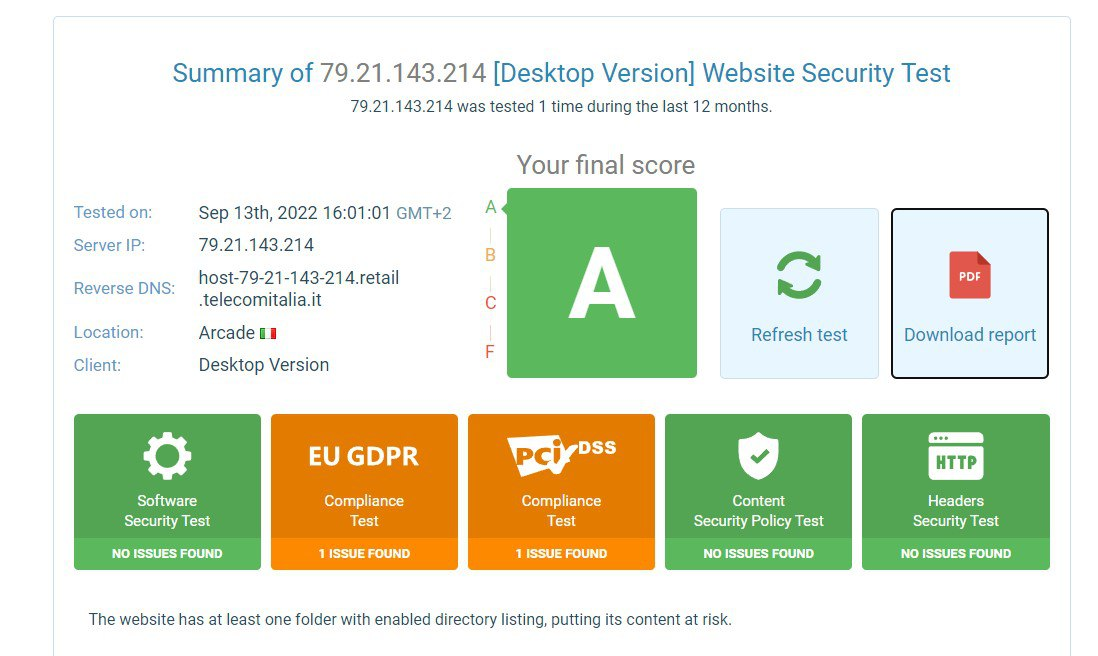
\includegraphics[scale=0.6]{Images/Sicurezza.jpg}
    \caption{Certificato di sicurezza}
    \centering
  \end{figure}

  Un altro punto a cui abbiamo prestato molta attenzione è la sicurezza. \\
  Deve essere garantita la sicurezza dei dati dell'utente. Per questo motivo, l’accesso all’account personale di un utente è protetto tramite credenziali salvate in una tabella dedicata nel DB, criptate tramite algoritmo SHA1 con aggiunta di sale. \\
  Per la registrazione, login e cambio password delle procedure sicure dedicate sono state salvate all’interno del DB. \\
  Tutte le funzioni per l’accesso e la scrittura dei dati nel DB sono contenute in un unico file DBAccess.php che agisce come ulteriore sicurezza controllando i dati immessi e usando prepared\_statements su ogni funzione. \\
  Ogni pagina controlla i dati forniti dagli utenti tramite filter\_var e non procede se tutti i campi sono inseriti e corretti. Inoltre, le pagine o moduli dedicati a funzioni usano un grande numero di controlli per verificare che ogni azione che un utente tenti di compiere sia valida. \\
  Se ad esempio un utente normale tenta di forzarsi dentro ad una parte amministrativa inserendo l’url specifico oppure tenta di compiere azioni su lavori o profilo non suoi come la cancellazione, l’azione viene bloccata e l’utente viene ridiretto alla pagina precedente con segnalazione di errore. \\
  È stato creato anche un file .htaccess dedicato per una migliore gestione e sicurezza del sito. \\
  Sono stati implementati vari headers per prevenire XSS, implementata una CSP, nosniff da parte di altre pagine web esterne al dominio, DENY bloccati i Frame per prevenire un altro sito di caricare JobFinder in modalità frame. Sono stati bloccati gli accessi a diversi domini noti come bots e infine un default Deny from all per tutti i file a cui l’utente non ha i permessi di interagire.
  È stato implementato ErrorDocument per gli errori 404 e 500. 
  Assieme al .htaccess è stato fornito anche un php.ini per la configurazione dei cookie sicuri, tuttavia non installato a causa della mancanza dei permessi di amministratore sulle macchine di laboratorio. Le password richieste devono essere lunghe almeno otto caratteri ed avere almeno una lettera maiuscola, una minuscola e una cifra. Il dominio dell’indirizzo e-mail inserito dall’utente è controllato se presente in una blacklist di noti domini finti o temporali, così da prevenire la facile registrazione di account spam/bot finti. La sicurezza del sito è stata testata manualmente attraverso diversi tools su OS Kali Linux e tramite tools online come www.immuniweb.com. 
  Il sito è quindi sicuro a diversi tipi di attacchi informatici come: Cross-site scripting (XSS), SQL injection (SQLI), Path traversal, Local file inclusion, Cross-site request forgery (CSRF),  XML external entity (XXE). \\
  È stata creata anche il file security.txt all’interno della cartella .well-known, un nuovo RFC 9116 che presto diventerà standard per la sicurezza di siti internet richiesta in tutti i siti web.